\chapter{Learning the parameters of a state-space model}
\label{chap:inference}

This chapter describes the state-space model (SSM) formulation we are working with. In \autoref{sec:ssm-definition}, we state our assumptions about the individual probability distributions. Then in \autoref{sec:parameter-inference}, we calculate the posterior distribution of the parameters of interest, and show that straightforward inference is not possible. Further on, we derive a sampler to approximate this distribution. By itself, this sampler is unusable, as it requires the evaluation of the model likelihood. To circumvent this, we introduce the particle filter in \autoref{sec:particle-filter}. This section gives the definition and some of the properties of the filter. Later in \autoref{sec:particle-filter-estimate} we show how to use the particle filter to estimate the likelihood, and argue that it does not affect the asymptotic properties of the sampler.

\section{State-Space Model definition} \label{sec:ssm-definition}
The state-space model, often also called the hidden Markov model (HMM) assumes a sequence of latent states $\left\{\bx_t\right\}_{t=0}^\infty \subseteq \R^{d_x}$ following a Markov chain, and a sequence of observed variables $\left\{\by_t\right\}_{t=1}^\infty \subseteq \R^{d_y}$. All involved distributions are parameterized by an unknown static parameter $\btheta \in \Theta \subset \R^d$.

For a fixed time $T \geq 1$, we use the shorthands $\bx_{0:T} = \left\{\bx_t\right\}_{t=0}^T$ and $\by_{1:T} = \left\{\by_t\right\}_{t=1}^T$.

The HMM formulation means that the joint distribution of $\bx_{0:T}$ and $\by_{1:T}$ factorizes, for any $T \geq 1$, into
\begin{equation}\label{eq:factorization}
p(\bx_{0:T}, \by_{1:T} \mid \btheta) = \sprior(\bx_0 \mid \btheta) \prod_{t = 1}^{T} \trans_t(\bx_t \mid \bx_{t-1}, \btheta) \obs_t(\by_t \mid \bx_t, \btheta),
\end{equation}
where $\sprior$ is the prior distribution over the initial state, $\trans_t$ is the transition distribution at time $t$ and $\obs_t$ is the observation model at time $t$.

The factorization \eqref{eq:factorization} can be written more clearly as
\begin{align}
\bx_0 \mid \btheta & \sim \sprior(\cdot \mid \btheta), \\
\bx_t \mid \bx_{t-1}, \btheta & \sim \trans_t(\cdot \mid \bx_{t-1}, \btheta), \quad t = 1, \ldots, T, \\
\by_t \mid \bx_t, \btheta & \sim \obs_t(\cdot \mid \bx_t, \btheta), \quad t = 1, \ldots, T.
\end{align}

Finally, in accordance with the Bayesian approach \citep{bayes}, we introduce a prior distribution $\pprior$ over the unknown parameters $\btheta$ quantifying our knowledge about $\btheta$ before observing any data. This allows us to state the full joint distribution
\begin{equation}\label{eq:full-joint}
p(\bx_{0:T}, \by_{1:T}, \btheta) = p(\bx_{0:T}, \by_{1:T} \mid \btheta) \pprior(\btheta).
\end{equation}
The corresponding graphical model is depicted in \autoref{fig:graphical-model}.
\begin{figure}[ht]
    \centering
    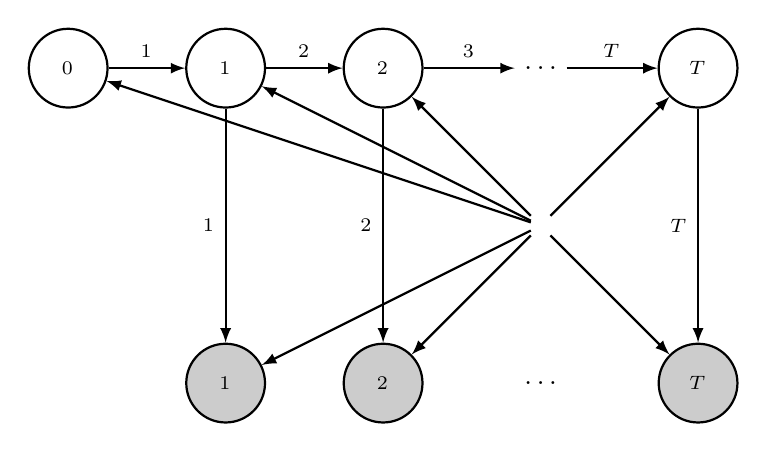
\begin{tikzpicture}
    % Style
    \tikzstyle{main}=[circle, minimum size = 10mm, thick, draw =black!80, node distance = 16mm]
    \tikzstyle{connect}=[-latex, thick]
    
    % Nodes X
    \node[main,shape=circle,draw=black](X0) at (1,4) {$\bx_0$};
    \node[main,shape=circle,draw=black](X1) at (3,4) {$\bx_1$};
    \node[main,shape=circle,draw=black](X2) at (5,4) {$\bx_2$};
    \node[](Xdots) at (7,4) {$\ldots$};
    \node[main,shape=circle,draw=black](XT) at (9,4) {$\bx_T$};
    
    % Node theta
    \node[](theta) at (7,2) {$\btheta$};
    
    % Nodes Y
    \node[main,shape=circle,draw=black,fill=black!20](Y1) at (3,0) {$\by_1$};
    \node[main,shape=circle,draw=black,fill=black!20](Y2) at (5,0) {$\by_2$};
    \node[](Ydots) at (7,0) {$\ldots$};
    \node[main,shape=circle,draw=black,fill=black!20](YT) at (9,0) {$\by_T$};

    % Edges XX
    \path [->] (X0) edge[connect] node[left] [above] {$\trans_1$} (X1);
    \path [->] (X1) edge[connect] node[left] [above] {$\trans_2$} (X2);
    \path [->] (X2) edge[connect] node[left] [above] {$\trans_3$} (Xdots);
    \path [->] (Xdots) edge[connect] node[left] [above] {$\trans_T$} (XT);
    
    % Edges XY
    \path [->] (X1) edge[connect] node[left] [left] {$\obs_1$} (Y1);
    \path [->] (X2) edge[connect] node[left] [left] {$\obs_2$} (Y2);
    \path [->] (XT) edge[connect] node[left] [left] {$\obs_T$} (YT);
    
    % Edges theta X
    \path [->] (theta) edge[connect] node[left] {} (X0);
    \path [->] (theta) edge[connect] node[left] {} (X1);
    \path [->] (theta) edge[connect] node[left] {} (X2);
    \path [->] (theta) edge[connect] node[left] {} (XT);
    
    % Edges theta Y
    \path [->] (theta) edge[connect] node[left] {} (Y1);
    \path [->] (theta) edge[connect] node[left] {} (Y2);
    \path [->] (theta) edge[connect] node[left] {} (YT);
    \end{tikzpicture}
    \caption{Graphical model describing the full joint distribution \eqref{eq:full-joint}. The shaded nodes denote the observed variables, white nodes represent the latent variables.}
    \label{fig:graphical-model}
\end{figure}

\section{Parameter inference} \label{sec:parameter-inference}

\section{The particle filter} \label{sec:particle-filter}

\section{Using the particle filter to estimate likelihood} \label{sec:particle-filter-estimate}